\documentclass{article}
\usepackage[utf8]{inputenc}
\usepackage[margin=0.75in]{geometry}
\usepackage{cite}
\usepackage{colortbl}
\usepackage{booktabs}% http://ctan.org/pkg/booktabs
\newcommand{\tabitem}{~~\llap{\textbullet}~~}
\usepackage[hidelinks]{hyperref}
\usepackage{subcaption}
\usepackage{graphicx}
\usepackage{titlesec}% http://ctan.org/pkg/titlesec
\titleformat{\section}%
    [hang]% <shape>
    {\normalfont\bfseries\Large}% <format>
    {}% <label>
    {0pt}% <sep>
    {}% <before code>
\renewcommand{\thesection}{}% Remove section references...
\renewcommand{\thesubsection}{\arabic{subsection}}%... from subsections
\usepackage{bookmark}
\usepackage{enumitem}
\usepackage{multicol}
\usepackage{mathtools}
\usepackage{lipsum}  
\setcounter{secnumdepth}{3} % default value for 'report' class is "2"


\DeclarePairedDelimiter{\ceil}{\lceil}{\rceil}
\usepackage[figuresleft]{rotating}

\begin{document}
\begin{center}

    % MAKE SURE YOU TAKE OUT THE SQUARE BRACKETS

    \LARGE{\textbf{COMP 3004 - Deliverable \#3 \\ System Architecture and Design}}\\ 
    % \vspace{1em}
    \Large{\href{https://github.com/alextrosta/brackit}{\texttt{Brackit}} - Mobile Tournament Bracket Creation} 
    % \vspace{1em}
    % \normalsize\textbf{Jaime Herzog, Suohong Liu, Xiyi Liu, Alex Trostanovsky} \\
    % \normalsize{
    %     \href{mailto:jaime.herzog@carleton.ca}{jaime.herzog@carleton.ca},
    %     \href{mailto:suohong.liu@carleton.ca}{suohong.liu@carleton.ca},
    %     \href{mailto:xiyi.liu@carleton.ca}{xiyi.liu@carleton.ca},
    %     \href{mailto:alex.trostanovsky@carleton.ca}{alex.trostanovsky@carleton.ca}
    % }\\
    % \normalsize{
    %     101009321,
    %     101002340,
    %     101004577,
    %     100984702,
    % }
    % \vspace{1em}
    % \normalsize{Carleton University, School of Computer Science} \\
\end{center}
% \begin{normalsize}

% \end{normalsize}

\section*{Metadata}
\subsection*{Team / App Name: \href{https://github.com/alextrosta/brackit}{\texttt{Brackit}}}
% \textbf{Team Member Names:}\\ Jaime Herzog: 101009321, Suohong Liu: 101002340, Xiyi Liu: 101004577, Alex Trostanovsky: 100984702


\subsection*{Team member names}
\begin{center}
    \begin{tabular}{ |l|c| }
        \hline
        \textbf{Name}     & \textbf{Student ID} \\
        \hline
        Jaime Herzog      & 101009321           \\
        Suohong Liu       & 101002340           \\
        Xiyi Liu          & 101004577           \\
        Alex Trostanovsky & 100984702           \\
        \hline
    \end{tabular}
\end{center}
\tableofcontents
\clearpage
\section{Architecture}
% identify, describe, and justify the architecture of your project (architectural style, design patterns) \\
% Outcome is a system architecture that supports the functional goals and non-functional attributes of your project 
\subsection{Description}
\subsubsection{Functional \& Non-Functional Requirements}
In developing \texttt{Brackit}, we set out to address an urgent need by tournament organizers and attendants to visualize, manage, and interact with double elimination
brackets on their mobile devices. At a high level, we committed to developing a product that will meet the following \textbf{functional requirements}:
\begin{enumerate}
    \item{Tournament Organizers (TO's) can create, host, maintain, and visualize double elimination brackets.}
    \item{Registerd \texttt{Brackit} Users, as well as Guests, can use the application to join created tournaments.}
    \item{\texttt{Brackit} will store and maintain user profiles that will describe users' history:
    \begin{itemize}
        \item{Matches won/lost}
        \item{Tournaments entered/created}
    \end{itemize}
    }
\end{enumerate}
In terms of \textbf{non-functional requirements}, we believed \texttt{Brackit} should be \textit{usable} on mobile devices. \texttt{Brackit} users should be able to:
\begin{itemize}
    \item{View and access all components (Brackets, Rounds, Matches) of a tournament on an Android device.}
    \item{Seamlessly enter tournament competitors to brackets on an Android device.}
\end{itemize}
% \subsubsection{Components and Connectors}
Conceptually, \texttt{Brackit} needed to support the creation and maintenance of the following \textit{components}:
\begin{itemize}
    \item{\textit{Tournament}: The highest level of abstraction utilized in Bracket creation. A tournament acts a \textit{container} for brackets. \texttt{Brackit} supports double-elimination tournaments, where competitors cease to be eligible to win the tournament after losing two matches \cite{wiki:det}.}
    \item{\textit{Bracket}: Given the number of entrants and their corresponding seeds (ranks), 
    Double elimination brackets dictate competitor matchups and the progression of competitors through the Winners and Losers brackets. 
    Brackets contain 
    a dynamic list of Rounds. }
    \item{\textit{Round}: Rounds contain a dynamic list of Matches.}
    \item{\textit{Match}: Matches pair the strongest and weakest (according to rank) players in a Round.}
\end{itemize}  
% To develop the interface between each of the components mentioned above, we decided to implement the following \textit{connectors}:
% \begin{itemize}
%     \item{}
    
% \end{itemize}
\subsection{Justification of Architectural Style Choices}
\subsubsection{Object-Oriented Architectural Style}
\label{sssec:ooas}
As described above, a Double Elimination Tournament mobile management application must maintain a set of well-defined entities (i.e. a Tournaments, Brackets, Rounds, and Matches) with predetermined relationships. For example, given $n$ competitors, a correct double elimination tournament will contain $\ceil{\lg n}$ rounds in the Winners bracket and $\ceil{\lg n} + 
\ceil{\lg \lg n}$ rounds in the Losers bracket. In addition, the progression of competitors can be calculated at the creation of a tournament, and handling this progression follows a deterministic approach (e.g. The winner of Match 1 of Round 1 in the Winners Bracket will always progress to Match 1 Round 2 in the Winners Bracket - see Figure \ref{fig:deb} for an illustrative example).\\
Therefore, to encourage an efficient decomposition of the algorithm and entities associated with Double Elimination Tournament creation, we decided to model the architecture of \texttt{Brackit} using an \textbf{Object-Oriented} (OO) architecture. 
Specifically, we chose to model each of the components of our application as objects. This allowed us to encapsulate the expected behaviour of each of the tournament objects while maintain a valid separation of concerns. To further explicate the validity of the choice of an OO architecture for \texttt{Brackit} consider the dynamic nature of Tournament creation.\\
A tournament bracket acts as a container for rounds, which themselves act as containers for matches.
To handle the progression of a competition, the data associated with each match (i.e. which competitor won or lost) should be self contained within the match object instantiation, but also must be accessible through attributes of that object. Therefore defining the Match construct as an object allows the definition of self-contained class methods and attributes that achieve these intended behaviours.
    \begin{figure}[htp]
        \centering
        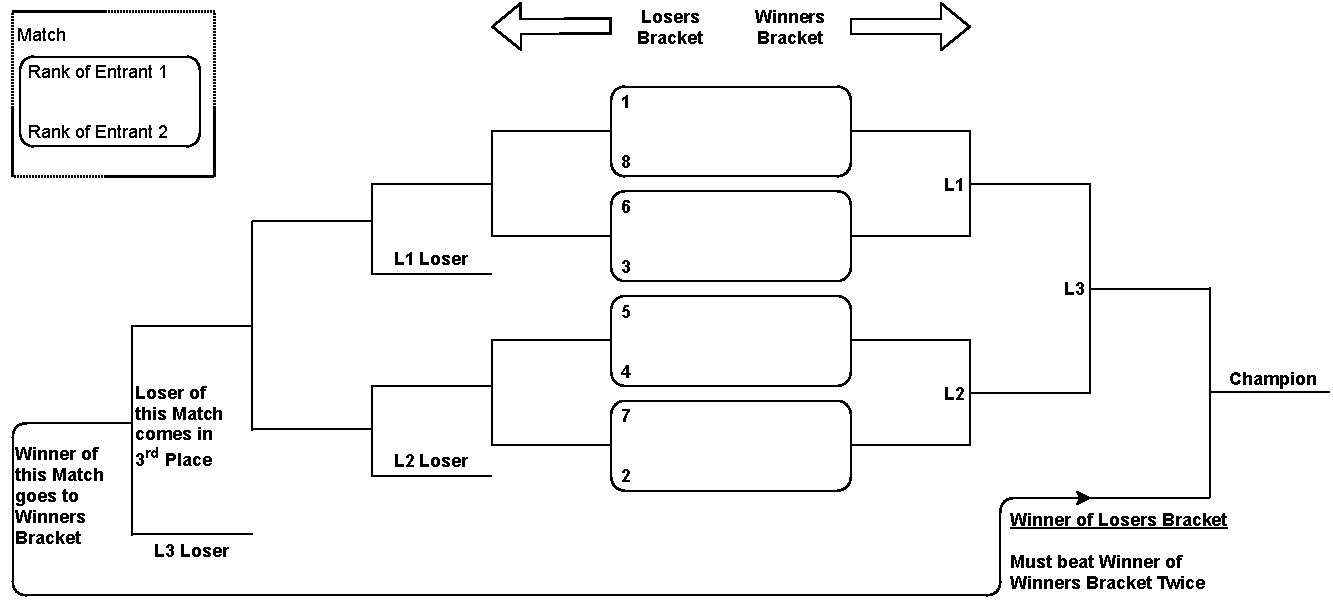
\includegraphics[width=12cm]{../diagrams/double_elim_bracket_comp.pdf}
        \caption{Seeded Double Elimination Tournament Chart for 8 competitors. (Adapted from \cite{se:tba})}
        \label{fig:deb}
        \end{figure}
\subsubsection{Client-Server Architectural Style}
\lipsum[2-4]
\clearpage
\subsection{Architectural Diagrams}
\vfill
\begin{center}
    \begin{figure}[htp]
        \centering
        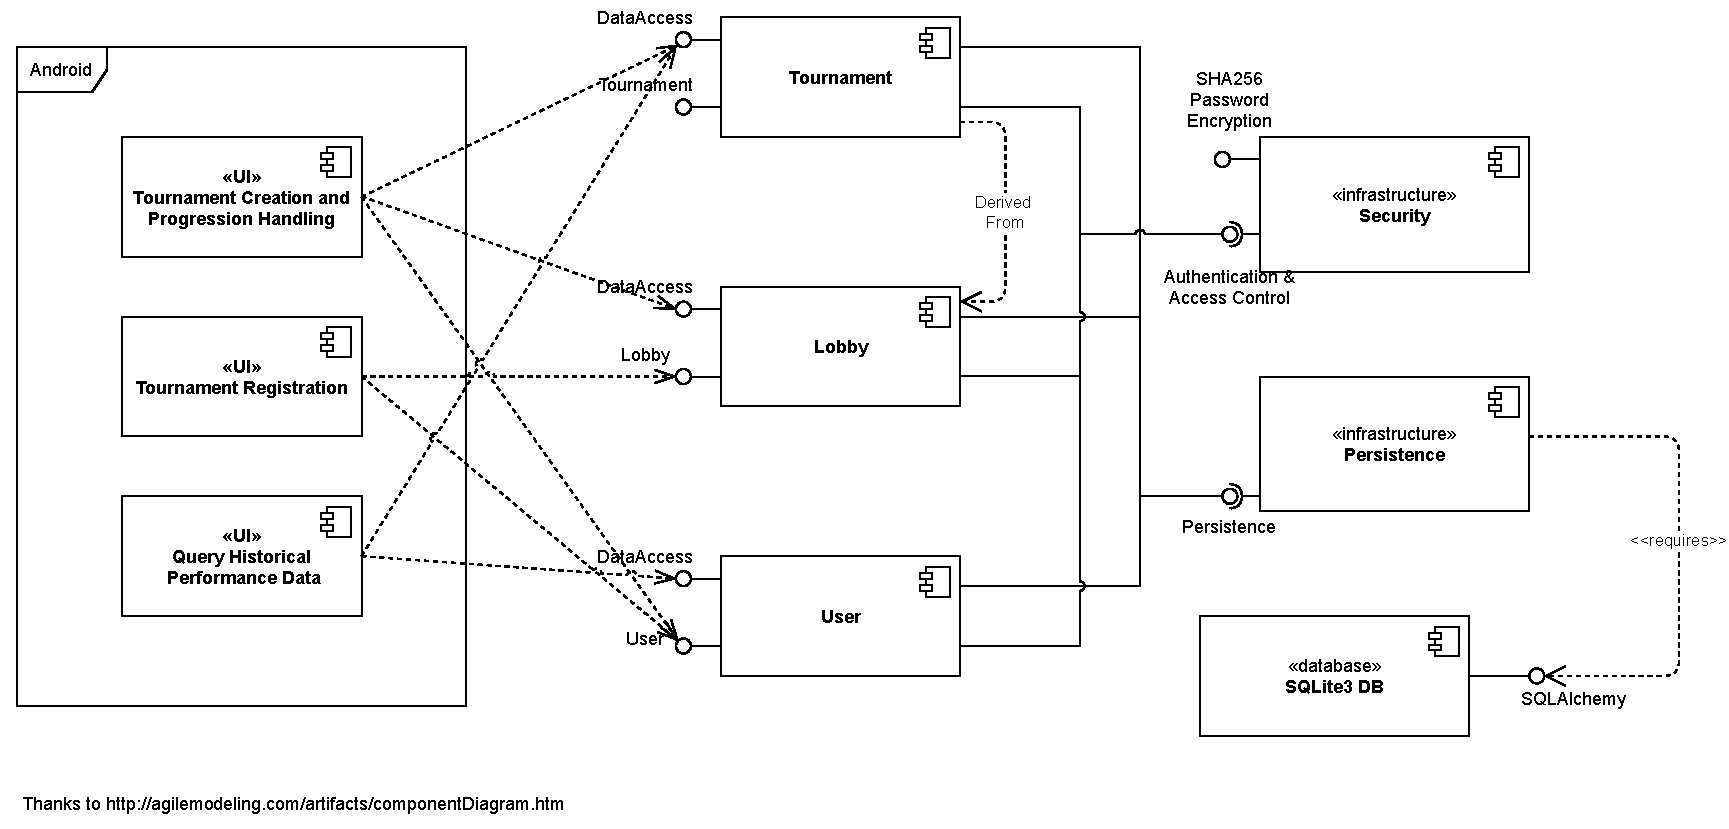
\includegraphics[width=14.5cm]{../diagrams/component_diag.pdf}
        \caption{\texttt{Brackit - }\href{https://sparxsystems.com/resources/tutorials/uml2/index.html}{UML 2} Architectural Component Diagram}
        \end{figure}
\end{center}
\vfill

\begin{center}
    \begin{figure}[h]
        \centering
        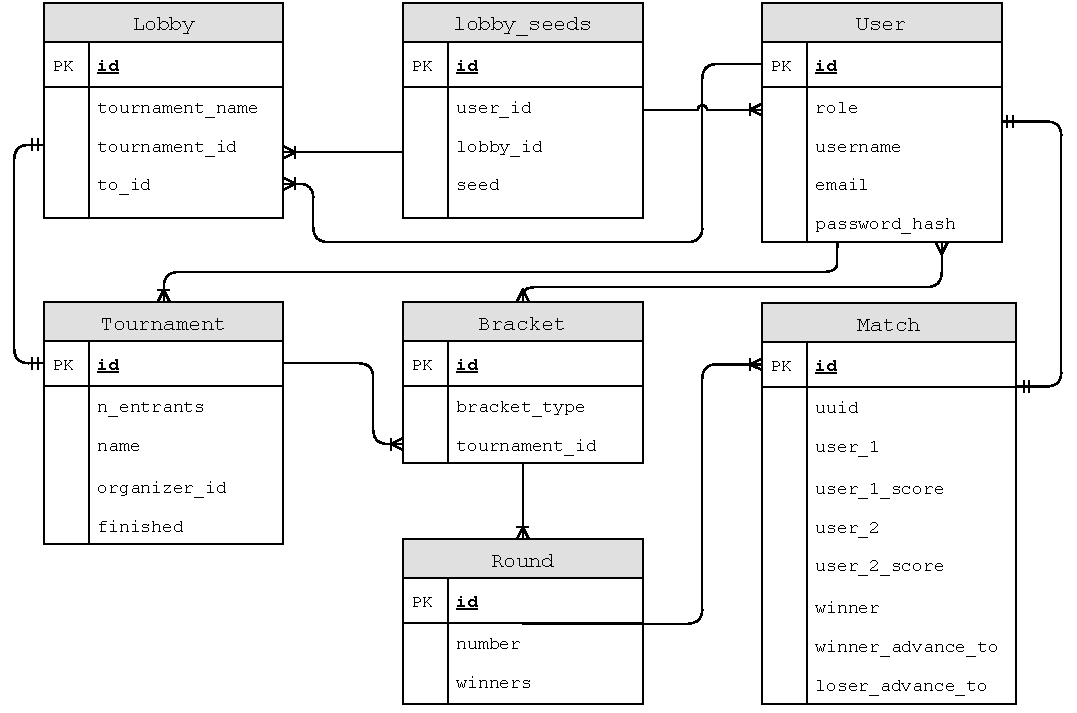
\includegraphics[width=12.5cm]{../diagrams/er_compressed.pdf}
        \caption{\texttt{Brackit - } Entity Relationship (ER) Diagram}
        \end{figure}
\end{center}
\clearpage
\section{Design}
\subsection{Description and Rationalization}
The \texttt{Brackit} backend was designed primarily to marry extensibility with the correctness of 
our relatively complex domain. The main challenge of the backend's design is the creation of 
correct brackets, as well as the maintenance of brackets as they progress to completion.

When we create a Tournament, we create a \href{https://github.com/alextrosta/brackit/blob/master/backend/tournament.py#L18}{tournament object} in the backend, which itself creates
the \href{https://github.com/alextrosta/brackit/blob/master/backend/tournament.py#L59}{bracket objects}. Depending on the bracket type, the appropriate number of rounds are created, 
with each round containing the corresponding number of matches. This is handled automatically because
the number of rounds is deterministic with respect to the number of entrants and the type of bracket (See Section \ref{sssec:ooas}).\\
So far, \texttt{Brackit} only supports double elimination brackets, but this can be expanded easily by the addition of special cases in the Bracket constructor. An alternative approach would be to create an abstract Bracket
class with each bracket type as an implementation of the abstract Bracket class. This may allow for 
code that is easier to read and iterate, and would be worth the refactoring time if this project were 
to be expanded on.

A specific implementation challenge is handling how each match knows who is the entrant which is playing 
in said match. This is called progression - for matches in the initial rounds, this is trivial as 
the entrants are simply placed into the matches when the Tournament is instantiated, but as the tournament
progresses, $\dots$

Our backend uses the \href{https://flask.palletsprojects.com/en/1.1.x/}{\texttt{Flask}} python package to expose our bracket and user information to 
the frontend, as well as \href{https://www.sqlalchemy.org/}{SQLAlchemy} to manage this information in the database. SQLAlchemy provides a \href{https://flask-sqlalchemy.palletsprojects.com/en/2.x/models/}{\texttt{Model}} baseclass that allows us to declare the tournament objects as database tables and a runtime interface by which we interact with our \href{https://www.sqlite.org/index.html}{\texttt{SQLite3}} database. We model each class in our class diagram in \href{https://github.com/alextrosta/brackit/blob/master/backend/app/models.py}{\texttt{models}} module, which creates 
tables for each class and defines the table relationships in an object oriented style. This 
allows us to easily and safely query the database itself when invoking APIs, and enables 
retrieval of the specific object being requested. Additionally, these models allow for 
seamless SQL querying for user data, such as users cross-tournament wins and losses. 

\subsection{Design Patterns}
\begin{enumerate}
    \item \textit{Facade}
    
    The Facade pattern intends to provide a unified interface to a set of interfaces in a subsystem. 
    For our backend, the API endpoints contained in the \href{https://github.com/alextrosta/brackit/blob/master/backend/app/routes.py}{\texttt{routes}} module constitute our Facade. Each endpoint provides a URL which the user can access
    to invoke all necessary interfaces to execute the necessary code in the backend.

    This pattern provides a singular hub through which frontend clients can access backend data,
    In addition, modelling our server as a Facade centralized all exposed endpoints and allowed for ease of use and extensibility.

    \item \textit{Singleton} 
    
    The Singleton pattern intends to ensure a class has only one instance, and to allow global 
    access to that class. The \texttt{Flask} app object leverages the Singleton pattern in its design, as 
    it is instantiated only once when the server is started, and is accessed globally throughout the 
    backend. 
    The justification for the use of the Singleton pattern for the app object is because the app 
    class itself, when instantiated, is the representation of the Flask server instance at compile time,
    and is how we modify and customize our server, i.e. specifying the database schema, or specifying the API 
    endpoints. Additionally, ensuring the app is only instantiated once maintains consistency throughout the session,
    as multiple apps could potentially create multiple duplicate endpoints, which would create unintentional behaviour
    such as the duplication of method invocation.
\end{enumerate}
\clearpage
\section{Design Diagrams}
\begin{center}
    \begin{figure}[htp]
        \centering
        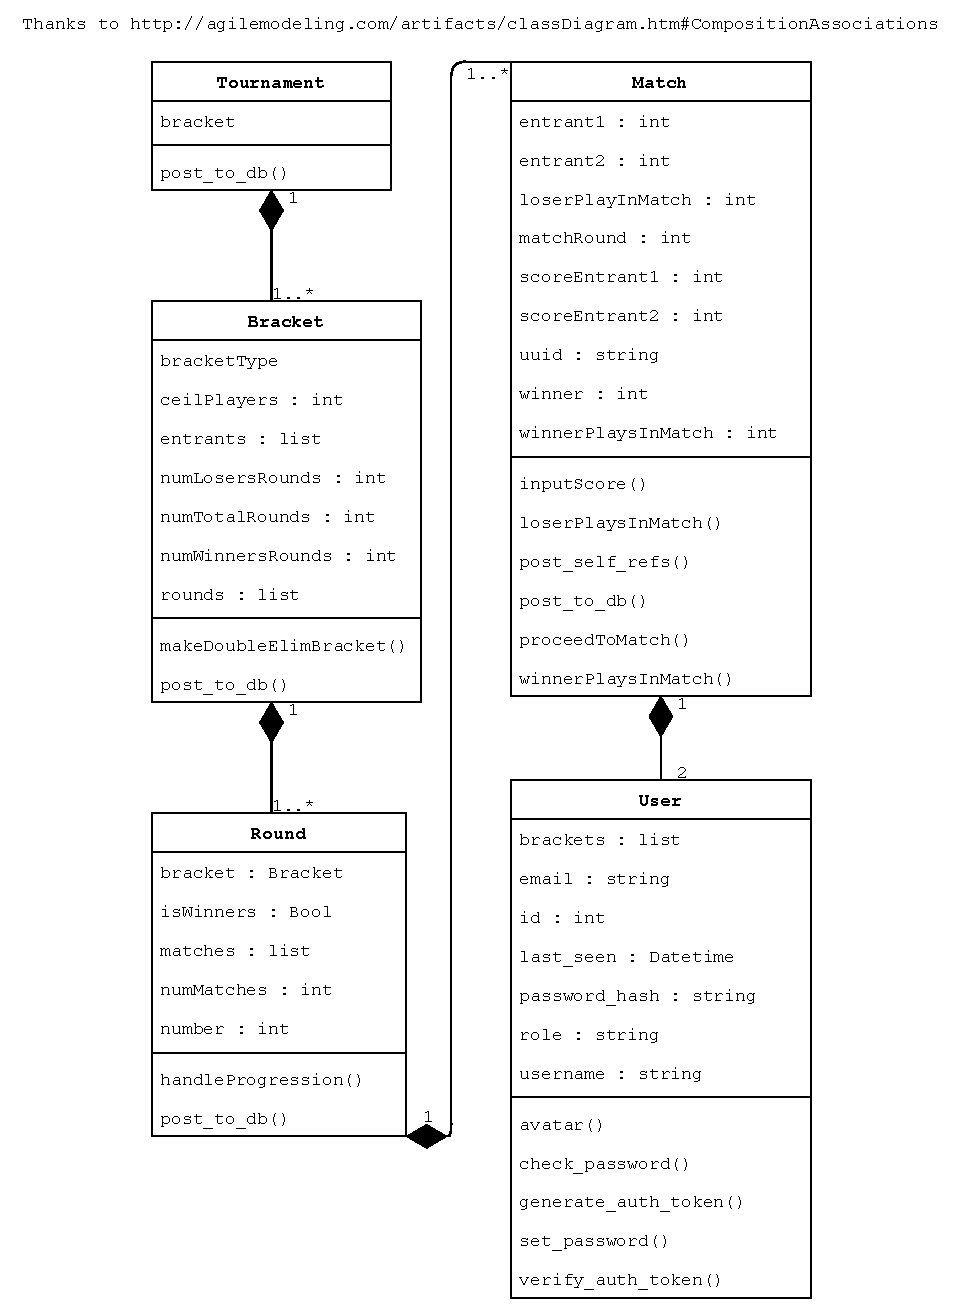
\includegraphics[width=13cm]{../diagrams/uml_class_tourn.pdf}
        \caption{\texttt{Brackit - }UML Class Diagram}
        \end{figure}
\end{center}



\clearpage
% \cite{wiki:xxx}
\bibliographystyle{unsrt}
\bibliography{ref.bib}


\end{document}